%%%%%%%%%%%%%%%%%%%%%%%%%%%%%%%%%%%%%%%%%%%%%%%%%%%%%%%%%%%%%%%%%%%%%%%%%%%%%%%%%%%%%
% Industrial implementations of RL
%
%
% 
%%%%%%%%%%%%%%%%%%%%%%%%%%%%%%%%%%%%%%%%%%%%%%%%%%%%%%%%%%%%%%%%%%%%%%%%%%%%%%%%%%%

This chapter starts with a literature review on the most famous RL applications in history.  Applications in this section have all been widely covered by the media and are well known amongst researchers and industrial practitioners alike.  Then, a review on RL applications catered towards the process control industry will be provided. Finally, this chapter is concluded with an impressive application of RL for power optimization. The main contribution of this chapter is the conducted literature view.

\section{Renowned triumphs}
The world witnessed, for the first time, artificial intelligence learning and playing games with a mere camera placed in front of the computer screen \cite{dqn1, dqn2}!  In this application, a general RL agent \textit{successfully} conquered various ATARI games using the camera images alone. However, such games are simple near-deterministic environments with sufficiently small state and action spaces, allowing even rules-based methods to be near-optimal (though previous algorithms did not \textit{learn} the games, nor can they play multiple games with the same algorithm). Although DQN showcased the power and generality of DQN, previous methods were already near-optimal in such simple environments. To conquer a task never done before by computers, Google DeepMind developed AlphaGo in 2016.  AlphaGo was an RL algorithm built to conquer Go, an ancient 2-player board game invented 3,000 years ago in China \cite{alphago1, alphago2}. Go is widely known as a near-impossible game for machines due to the insane dimensions of its state and action space (over $10^{170}$ possible states, a googol times larger than Chess), and the requirement to defeat opponents with stochastic strategies. State-of-the-art Go programs struggle against even amateur players; however, AlphaGo decisively defeated Ke Jie, the world's best Go player. The structure of AlphaGo employs \textit{value networks} to evaluate the board state. Then, \textit{policy networks} are used for optimal action selection.  During initial training, the agent used supervised learning to gain fundamental knowledge from amateur level play.  Afterwards, advanced strategies were developed by learning from expert level play.  After surpassing the experts, the agent continued to \textit{perfect} itself through conducting playing against itself, ultimately evolving into the world's best Go player in history \cite{alphago1, alphago2}. In terms of real world applications, these experiments demonstrate the potential of RL to identify new techniques and insights to advance modern engineering beyond what is already known.

Originally, AlphaGo contained human engineered features that were initially believed to enhance the agent's learning speed. Ironically, DeepMind throught the complete opposite.  Instead, DeepMind believed that the features actually handicapped the agent's skill ceiling, leading to the development of AlphaGo Zero (zero refers to zero engineered features), an more natural version of AlphaGo that is free of human intervention \cite{alphagozero}. In AlphaGo Zero, the states were simply the locations of the black and white stones. In terms of the algorithm, AlphaGo Zero combined the value and policy networks into one network, making it a more simple algorithm. After training for approximately 40 days starting \textit{tabula rasa}, AlphaGo Zero was able to surpass AlphaGo through pure self-play, without human engineered features or learning fundamentals from human play. Furthermore, just 3 days was needed for AlphaGo Zero to achieve world championship level (i.e., the level required to decisively defeat Ke Jie). AlphaGo Zero was also much more efficient, using only 4 tensor processing units (TPUs) compared to the 48 used by AlphaGo resulting in a 90\%+ reduction in energy usage.

In the latter half of 2017, AlphaGo Zero was perfected into AlphaZero, a general RL algorithm capable of teaching itself Chess, Shogi, and Go.  Additionally, the agent was ultimately able to defeat the world champion program in each respective case \cite{alphazero1, alphazero2, alphazero3}. Architecturally, AlphaZero uses a deep neural network $(\textbf{p}, v) = f_{\theta}(x)$ where $\textbf{p}$ represents a vector of action probabilities $p_u = Pr(u|x)$, $\theta$ are the parameters of the neural network, and $v \approx \mathbb{E}[z|x]$ where $z$ denotes the expected game outcome \cite{alphazero3}. For example, $z$ = -1 for a loss, 0 for a tie, and 1 for a win. Magnus Carlsen, the world's best Chess player in history, had a peak FIDE ELO (skill evaluation assigned by FIDE, the world's most prestigious Chess organization) of 2882.  In Chess programs using supervised learning to replicate Mr. Carlsen's playstyle, the ideal agent would be hard capped at 2882, a level representing zero replication error. Comparatively, AlphaZero achieved an ELO above 3300 from pure self-play in just 200,000 training steps. In 300,000 training steps (4 hours physical time), AlphaZero confidently surpassed Stockfish, the best Chess engine \cite{stockfish}.  Comparing AlphaZero with Stockfish, Stockfish required \textit{decades} of careful engineering and refinement by Chess and software experts.  AlphaZero started knowing literally nothing, and after 4 hours of self-play, it was crowned the best Chess player in history. The most impressive accomplishment of AlphaZero in a RL literature contribution sense is the demonstration of RL's ability for long-term decision making. That is, AlphaZero played Chess like no other.  The agent started by sacrificing many pieces in the early game to eventually obtain a significant advantage in the end game, some thirty steps in the future. Furthermore, AlphaZero only needs to search $10^4$'s moves per turn compared to traditional Chess engines, like Stockfish, where up to $10^7$'s moves are searched (over 1000 times more!). More impressively, AlphaZero was then used to learn Shogi and Go as well. Ultimately, the agent was able to defeat the respective best game engines, Elmo and AlphaGo Zero.

The achievements of DQN, AlphaGo, AlphaGo Zero and AlphaZero are all technologically amazing; however, all previous applications hold no true value in the real world.  More specifically, the algorithms were all applied in a \textit{perfect information} system where all system states are perfectly observable and without stochasticity.  For example, you cannot keep the location of your pieces hidden from your opponent in Chess. Additionally, the applications did not require real-time decision making. Instead, the computers were given excessively long periods of time to provide an action. Comparatively, systems in the real world occasionally contain fast dynamics and often contain unobservable, and/or unreliable information. To demonstrate RL's ability to perform in stochastic and partially observable settings similar to the real world, AlphaStar was developed \cite{alphastar}. Here, the agent learned to play StarCraft II, a \textit{real time} strategy game where the player acts as the general of an army.  Here, the agent is tasked with optimally allocating sufficient resources for military and resource-generation needs in order to defeat the opponent. Compared to other games, StarCraft is a very difficult (most humans cannot properly play it), real time, and the opponent's moves are \textit{hidden} and, often times, \textit{stochastic} because the opponent is stochastic. The state and action spaces are also nearly infinite because of the wide range of available choices (much like a military general's job in real life). Here, the agent must respond and act fast enough to win real time battles while also managing the long term resource requirements of its army. In the past, ML methods were applied on \textit{simpler} real time games such as Mario or Quake with heavy simplifications. Even with such modifications, no algorithms ever performed even remotely close to professional level play.  In AlphaStar's case, the agent \textit{decisively} defeated two of the best StarCraft II pros using pixel inputs alone and on the full game (with no modifications). Moreover, AlphaStar was not given any additional hidden information and was also constrained to be inline with human capabilities (e.g., the agent is not allowed to perform thousands of actions per second, etc.). Through AlphaStar, RL was shown to have the ability to react to unexpected situations in real time high dimensional environments.  Additionally, RL was very successful in hierarchical long-term planning tasks, as shown by its ability to manage long-term resource needs.  Such characteristics are vital in industrial process control, especially in applications regarding fault-tolerant control or high dimensional multi-variate optimal control.

AlphaStar used an \textit{off-policy} actor-critic RL algorithm. Initially, AlphaStar learning fundamental strategies of StarCraft using supervised learning from previous game footage because the game is too difficult to learn \textit{tabula rasa}.  Afterwards, it conducted self play to perfect itself.

All applications above assumed a single agent environment.  In industrial process control, the agent must also identify the consequences of its actions on the entire process. RL's capabilities in multi-agent partially observable settings was first confidently demonstrated by OpenAI on a game known as Defense of the Ancients (DotA) 2. DotA, like StarCraft II, is a real time high dimensional strategy game (more commonly known as multiplayer online battle arena) where each \textit{team} tries to overcome the opponent. Unlike StarCraft, five players are on each team for DotA and all players must work together. In such a setting, the agent's interaction effects with other agents must be explicitly considered to identify the optimal policy. In DotA, the time horizon per game is also dramatically increased and can be up to 80,000. Comparatively, a game of Chess or Go typically ends within 150 turns \cite{openai}. In OpenAI Five, all agents use the proximal policy optimization algorithm and handles the system's partial observability using recurrent neural networks. At each time $t$, 20,000 continuous observations are provided to the agent.  The agent then picks 1 action out of 1,000 different actions. The agents' reward function contains two parts: individual performance and team performance. The team performance reward function was used to enhance cooperation among the independent agents.  In the reward function, a hyper parameter called \textit{team spirit}, denoted here as $\phi$, was used to imply the importance of individual and team performance.  Throughout each game, team spirit was annealed from 0 to 1 to establish that in the end game, only team performance matters. The reward function for each agent is:
\begin{equation}
    r(x, u) = \phi \cdot \text{team reward function} + (1 - \phi) \cdot \text{individual reward function}
\end{equation}
On April 2019, OpenAI Five defeated the world's highest ranked DotA 2 teams \cite{openai2}.

Modern RL debuted in near-deterministic low dimensional video games, eventually transitioning to more complex systems that reflected the uncertain, unobservable, and stochastic nature of the real world.  Throughout all these modern RL triumphs, RL agents was shown to have capabilities to optimally handle partially observable, long horizon, and high dimensional systems (better than humans).  Additionally, RL has fast online evaluation times, allowing for quick reactions to unexpected situations.  RL can also learn the optimal policy in multi-agent systems and is feasible for real time applications with exceptionally fast dynamics. Most critically, RL was shown, time and time again, to be a general algorithm with the ability to learn different things. Such a characteristic could significantly reduce R\&D costs for advanced applications in industrial process control.



\section{Simulated RL Applications}
\subsection{RL for Adaptive PIDs}
Initially, senior management might hesitate to implement RL for direct closed loop control due to safety concerns. To gain initial approval, this section introduces RL methods to optimally tune PIDs.  Proportional-Integral-Derivative (PID) controllers are widely used throughout many processes due to their simplicity, effectiveness, and ease of implementation. The general PID formulation is given by \cite{process_control_ref13}:
\begin{equation}
    u(t) = K_p \varepsilon(t) + K_i \int\limits_{\tau = 0}^T \varepsilon(\tau)dt + K_d\dot{\varepsilon}(t)
\end{equation}
where $\dot{\varepsilon}(t)$ denotes the change in error at time $t$. $K_p$, $K_i$, and $K_d$ are the PID parameters corresponding to the proportional, integral, and derivative gain, respectively.  These parameters must be \textit{well tuned} for optimal controller performance; however, the tuning process is time-consuming, especially in MIMO systems with many interacting control loops (i.e., proper tuning of one control loop ends up de-tuning another).  Many traditional approaches exist for PID tuning.  One popular method is the Ziegler-Nichols method. But PIDs tuned using these general approaches typically perform well below optimal \cite{pid1}.  Here, RL agents will be used to automatically and optimally tune the PID parameters, resulting in superior performance while reducing engineering work hours.

Perhaps the earliest study on automated PID tuning using RL concepts was published in 2000 by \cite{pid1} (algorithm overview shown in Figure \ref{fig: CARLA}).  Application-wise, the authors was able to successfully tune a Ford Motors Zetec engine. The algorithm was called Continuous Action Reinforcement Learning Automata (CARLA), and was typically used for \textit{fine tuning} PIDs after initial parameters were set using methods like Ziegler-Nichols. Controllers tuned using CARLA resulted in a 60\% reduction in the cost function compared to traditional tuning methods.  CARLA is implemented as follows: Initially, each hyper parameter ($K_p, K_i, K_d$) corresponds to one CARLA.  The output of each CARLA is the recommended new hyper parameter and is picked from the corresponding probability density functions, $f(x)$.  For example, in a single PID system, there would exist three CARLAs corresponding to $K_p, K_i, \text{ and } K_d$. At each time step, the recommended parameters are outputted and is implemented into the PID.  Afterwards, the cost function using the recommended parameters is evaluated.  Costs lower than the mean will shift the distribution towards the recommended parameters, vice versa for higher costs. Exploration-wise, Gaussian white noise is added to the recommended parameters. Lastly, CARLA is typically applied to low dimensional settings due to its non-scalability nature. For more detailed information regarding CARLA, see \cite{pid1}.

\begin{figure}[H]
    \centering
    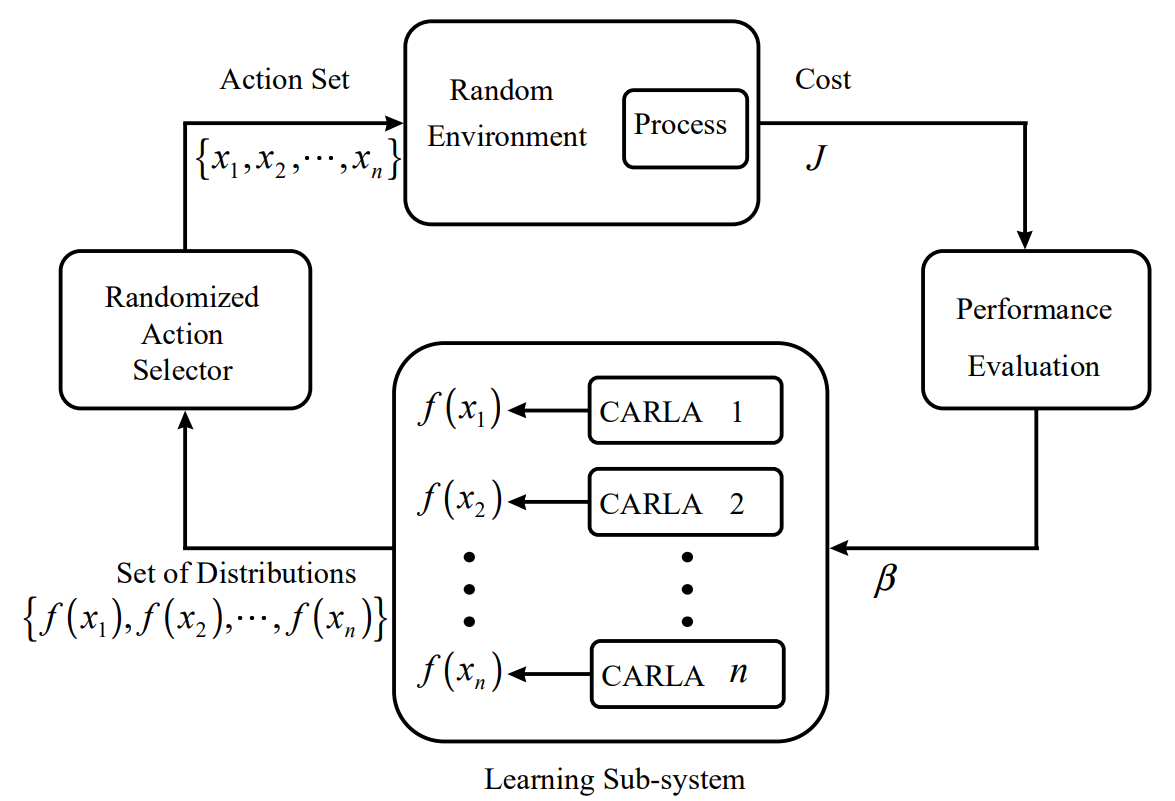
\includegraphics[width=0.55\textwidth]{images/ch5/CARLA.jpeg}
    \caption{CARLA: An RL-powered automatic PID tuning algorithm}
    \label{fig: CARLA}
\end{figure}

Six years later, \cite{pid2} developed a more sophisticated PID tuning approach through an actor-critic algorithm.  Here, the agent's states are given as:
$$x = [\varepsilon_t, \Delta \varepsilon_t, \Delta^2 \varepsilon_t]$$
$$\Delta \varepsilon_t = \varepsilon_t - \varepsilon_{t-1}$$
$$\Delta^2 \varepsilon_t = \varepsilon_t - 2\varepsilon_{t-1} + \varepsilon_{t-2}$$
and the actions are:
$$u = [K_i, K_p, K_d]$$
The states correspond to the integral, proportional, and derivative error terms of a discrete PID. Intuitively, the agent maps the current error, and the first- and second-order difference of errors to the optimal PID parameters at each $t$. Using the new parameters, the PID is re-parameterized and outputs $\Delta u_t$ using:
\begin{equation}
    \Delta u_t = K_i \varepsilon_t + K_p (\varepsilon_t - \varepsilon_{t-1}) + K_d (\varepsilon_t - 2\varepsilon_{t-1} + \varepsilon_{t-2})
\end{equation}
where $K_i, K_p,$ and $K_d$ are provided by RL and may change for each time $t$. From $\Delta u_t$, $u_t$ is calculated using:
$$u_t = u_{t-1} + \Delta u_t$$
From \cite{pid2}, results showed the algorithm's capability to near-perfectly track complex non-linear systems. By 2008, \cite{pid3} applied this algorithm onto an industrial wind turbine experiment, yielding near perfect set point tracking.  Applicational details are in \cite{pid3}. In 2015, the algorithm was implemented on an under-actuated robotic arm \cite{pid4}. Here, the system contains fast dynamics and lacks sufficient actuators for control. This study explores the RL tuning method's fault tolerant characteristics due to the under-actuated system.  To test the PIDs, the robotic arm had to maintain proper formations and was exposed to many disturbances. Traditionally tuned PIDs overshoot and exhibit other undesired behaviours; however, the RL tuned PID showed significantly better performance for disturbance rejection and response time. By 2017, a $Q$-learning variant of this algorithm was used to tune a race track robot \cite{pid6}.  Compared to PIDs tuned using traditional approaches, the robots tuned using RL achieved up to 59\% faster lap times. 

In 2013, \cite{pid6} introduced a new automated tuning strategy to tune robots playing soccer.  This new method was comparable to the one used for the multi-PID soccer robot. The main difference was the agent's states.  Instead of errors, the agent received the location of the robot in the soccer game. Intuitively, this gave the agent information regarding its current situation within the game, and allowed RL to tune its specifications accordingly.  For example, the robot will require faster speed when sprinting down the soccer field compared to when it is ready to score a goal. Such a tuning method may be useful for an event triggered control system in industry.  For example, if there is snow outside, the control system should act more conservatively and have less gain compared to normal ambient conditions. In \cite{pid6}, it was demonstrated that the RL tuned robots were vasting superior to robots tuned using the Ziegler-Nichols method.

RL was also used for a model-based PID tuning strategy where the controller's finite horizon cost was considered instead of its immediate tracking error. In the end, this method was highly successful and even worked on non-linear MIMO systems with arbitrary couplings. The method was validated in real life on a robot named Apollo.  Apollo had imperfect low-level tracking controllers and unobserved dynamics, but was able to perform adequately using the RL tuned PIDs. Advanced details regarding this implementation can be found in \cite{pid7}.

In recent literature, many more RL automated PID tuning methods were published, but were not listed here. Ultimately, all the "new" approaches are very similar to the ones presented with only slight alterations of the tuning set-up.















\subsection{RL in Process Control}
Studies where RL agents were applied solely for regulation or set-point tracking are still quite rare due the undeniable success of traditional methods. \cite{pc} was the first instance where RL was used for set-point tracking of an industrial process. Here, the authors tracked the set-point of a CSTR using a neural network based agent. In more recent literature, \cite{pc1} was the first to show deep RL's (DDPG) capabilities in process control.  Here, it was shown that RL can successfully control arbitrary SISO and MIMO systems as long as the reward function is properly established.  In \cite{pc1}, the agents mapped $x = [y_t, y_{sp}]$ to $u = [u_t]$. Intuitively, the states provided the current tracking error to the agent while the action changed the control input to mitigate the error. In \cite{pc2}, an actor-critic agent was used to regulate the temperature of a building heating, ventilation, and air conditioning (HVAC) system. Ultimately, the agent resulted in a 2.5\% reduction in energy consumption while achieving a 15\% increase in thermal comfort. The HVAC system was optimized again in \cite{pc3}.  This time, a proximal actor-critic RL agent was used. All previous applications formulated the agent to perform set-point tracking; however, there already exists many highly capable controllers for set-point tracking such as PIDs and MPCs. RL's greatest advantage compared to previous methods are its flexibility and ease of use for optimal control (i.e., optimize an economic objective). More specifically, optimal control can be achieved by simply changing the reward function to be in terms of an economic objective. Furthermore, RLs are also shown to be effective in fault-tolerant control (FTC) \cite{ftc}. Traditional FTC methods require modelling of all possible faults and is nearly impossible. Instead, an RL agent trained under different faults can identify a fault-robust optimal policy directly. Moreover, RL's \textit{model-free} nature and direct adaptive characteristics allow the agents to mediate faults even when trained on inaccurate process models and can also adapt to process drift.













\subsection{RL for Anomaly Detection}
Another field where RL gained traction is \textit{time series} anomaly detection. In industry, anomaly detection is a proactive application to identify potential hazards \textit{before} a loss incident occurs. Compared to previous methods, RL's ability to self-learn provide an attractive edge. \cite{seq_anomaly1} was perhaps the earliest paper to introduce RL-based anomaly detection (architecture shown in Figure \ref{fig:anomaly_detection}). Here, the authors built an adaptive neural network agent to identify cyber threats. Comparatively, the architecture is nearly identical to the time-series anomaly detection introduced in Chapter 3.  A POMDP was used to describe the system where the agent mapped observations $o = [x_{t-n}, x_{t-n+1}, ..., x_{t}]$ to actions $u = [\text{Normal }, \text{ Anomalous}]$, guided by a reward signal based on the success or failure of its last prediction. The reward function is designed as follows: correct identifications yielded +1 reward while misclassification yielded -1 reward. Notice that the observations were augmented past states. By doing so, the agent is provided with time-series information. More recently, Zighra (a online security company) deployed the algorithm from \cite{seq_anomaly1} into production through a software called SensifyID. Although the concepts here was originally proposed for networks; the same concept was shown in \cite{ftc} to work as a general fault detection tool for industrial process control as well.

\begin{figure}[H]
    \centering
    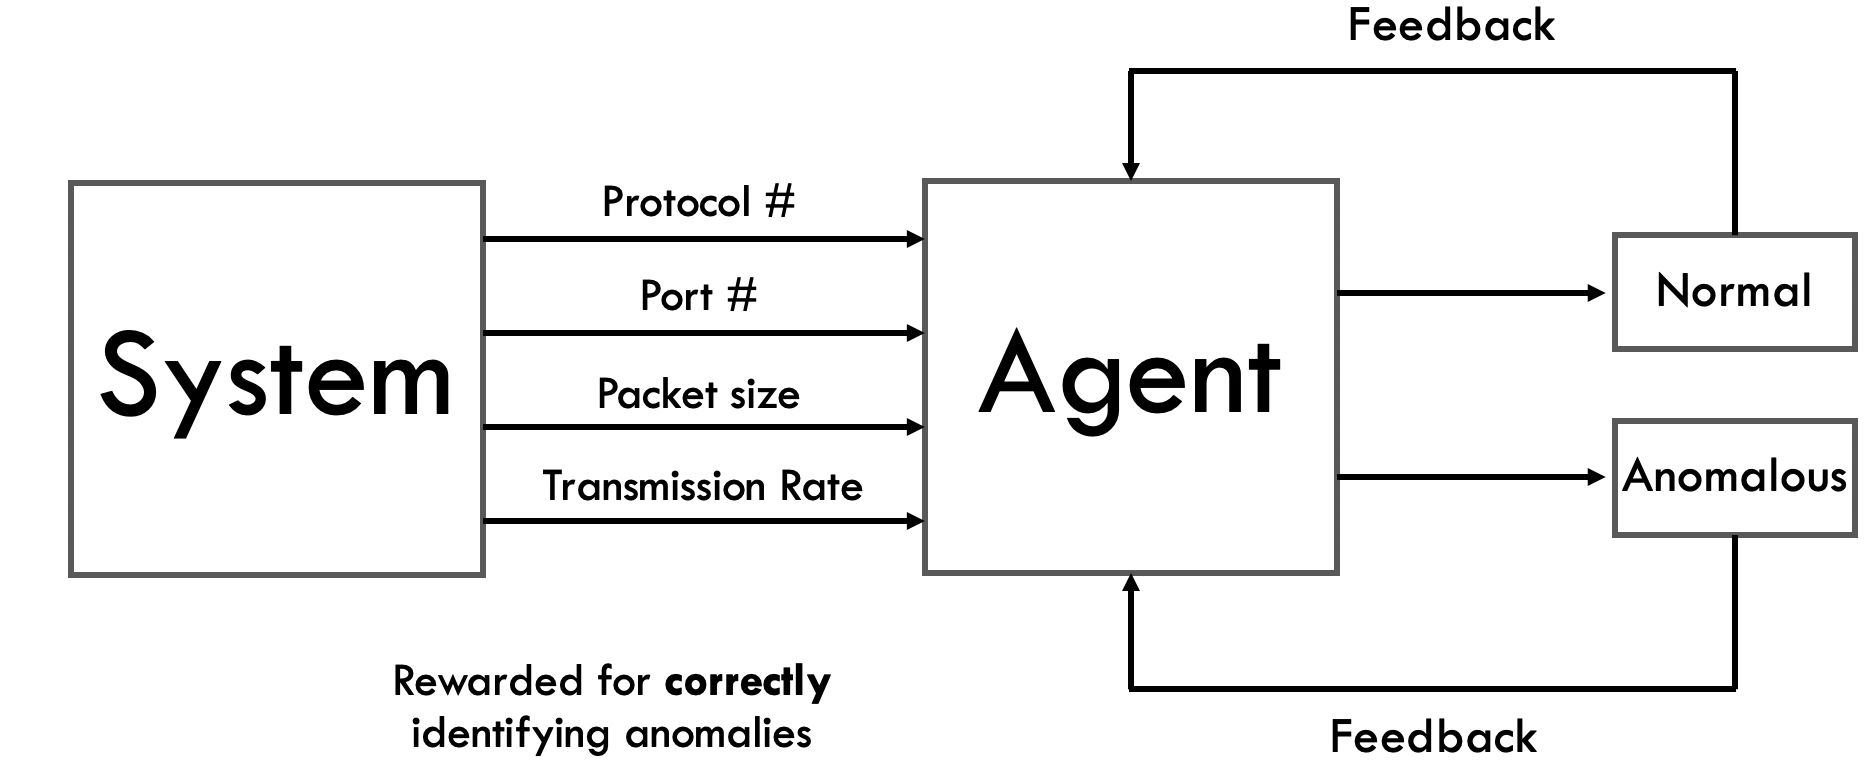
\includegraphics[width=0.7\textwidth]{images/ch5/anomaly_detection.jpeg}
    \caption{A sample anomaly detection architecture.}
    \label{fig:anomaly_detection}
\end{figure}   

In early 2010, \cite{seq_anomaly2} extended the original RL anomaly detection concepts by representing the system as a partially observable Markov \textit{reward} process (MRP). The states in this new algorithm remained $o = [x_{t-n}, x_{t-n+1}, ..., x_{t}]$. The agent had no actions since a MRP was used to represent the system. Instead, the agent learned the probabilities of each state transitioning into an anomalous state. Mathematically, this is given as:
\begin{equation}
    P_a(x) = P\{o_{t+1} \in \mathcal{A} | o_t\}
\end{equation}
where $P_a(x)$ represents the probability of transitioning into an anomalous state $a \in \mathcal{A}$ given observation $o_t$ where $\mathcal{A}$ is the set of anomalous states. There exists another hyper parameter, $\mu_a$, that denotes the anomaly threshold. High values reduce false positives but increase false negatives, while low values increase true positives but also increase true negatives. At any time when $P_a(x) > \mu_a$, an anomaly was deemed imminent. The value function of this approach is represented as:
\begin{equation}
    V(x) = \sum\limits_i^n P(o_{t+1} \in \mathcal{A} | o_t) \cdot r(o_t)
\end{equation}
where $r(o_t)$ is the reward received given $o_t$. If $o_t \in \mathcal{A}$, $r(o_t) = 1$, otherwise 0. Notice here that higher value states have higher chance of being anomalous. As validation, the authors compared the RL anomaly detection algorithm to other popular classification algorithms such as support vector machines. In the end, RL anomaly detection resulted in the highest detection accuracy, although all algorithms scored accuracies above 99.8\% on the selected data sets, even linear methods such as logistic regression \cite{seq_anomaly2}.
 
In 2018, Huang el al. introduced a recurrent neural network (RNN) based RL anomaly detection algorithm without needing to tune $\mu_a$ \cite{seq_anomaly3}. The algorithm was similar to \cite{seq_anomaly1} where $\pi(u, x)$ mapped states to actions $u = [\text{Normal }, \text{ Anomalous}]$.  In this representation, $\mu_a$ was not required because the classification is binary (i.e., not a probability). Compared to \cite{seq_anomaly1}, the new algorithm was still a POMDP; however, it used a long short term memory (LSTM) recurrent neural network (RNN) to memorize previous states rather than augmenting the previous states directly. The performance advantages between the two approaches have yet to be explored in literature, but the LSTM RNN should require significantly more training. The algorithm was validated on the Yahoo anomaly detection benchmark data set \cite{yahoo} and successfully identified all anomalies with no false alarms.














\section{Google's success story}
A world-changing implementation of RL was demonstrated by Google when a RL agent\footnote{Google DeepMind did not explicitly state the technology used to achieve the savings, only machine learning. However, DeepMind is a company that focuses on reinforcement learning approaches and there were many mentions of creating a general algorithm for all the data centers in the article; therefore, it was assumed reinforcement learning was used. More specifically, meta-RL was most likely used due to the construction of many simulators and the agent's adaptation speed.} showed the capabilities to autonomously controlling a \textit{live} data center, reducing electricity usage by up to 40\%. This also indirectly reduced the carbon footprint of all individuals using Google's services, which encompasses a large part of the world. Google's data centers generate enormous amounts of heat through powering services such as Google Search, Gmail, and YouTube. Hence, the data centers' primary energy usage is for cooling. Cooling industrial processes are accomplished by equipment such as heat exchangers, pumps, and cooling towers---even at Google.  Modelling such a complex, non-linear systems poses several difficulties, rendering traditional methods ineffective \cite{google_data1}:
\begin{enumerate}
    \item Complex, high-dimensional environment with uncountable non-linear interactions rendering modern system identification methods infeasible. Additionally, experienced human operators simply cannot comprehend the countless interactions.
    \item Highly dynamic internal and external building conditions (such as ambient temperature, server load, etc.) rendering rules- and non-adaptive methods intractable.
    \item All data centers have unique layouts and set-ups.  This non-consistency demands custom-tuned models for each individual data center, assuming traditional approaches were used; however, such a dilemma could be adequately overcame through artificial general intelligence where one algorithm can learn many different scenarios.
\end{enumerate}
To overcome these difficulties, DeepMind researchers first identified neural network models corresponding to different operating conditions by leveraging historical operating data from different data centers.  The inputs to the neural network models were sensor information such as temperature, pump speeds, ambient temperature, etc. The model output was the power usage effectiveness (PUE) given by:
\begin{equation}
    PUE = \frac{\text{Total building energy usage}}{\text{IT energy usage}}
    \label{eq:pue}
\end{equation}
Here, the neural networks were used as training simulators for the data centers. RL was applied on said simulators to learn a control policy to minimize the PUE. Different agents were trained on different data centers, during different operating conditions. When implemented, the ideal agent would be picked based on the current operating condition. Initially, the control actions provided by the agent were only recommendations.  The PUE with and without implementing the agent's recommendations is shown in Figure \ref{fig:google_data_center}.

\begin{figure}[H]
    \centering
    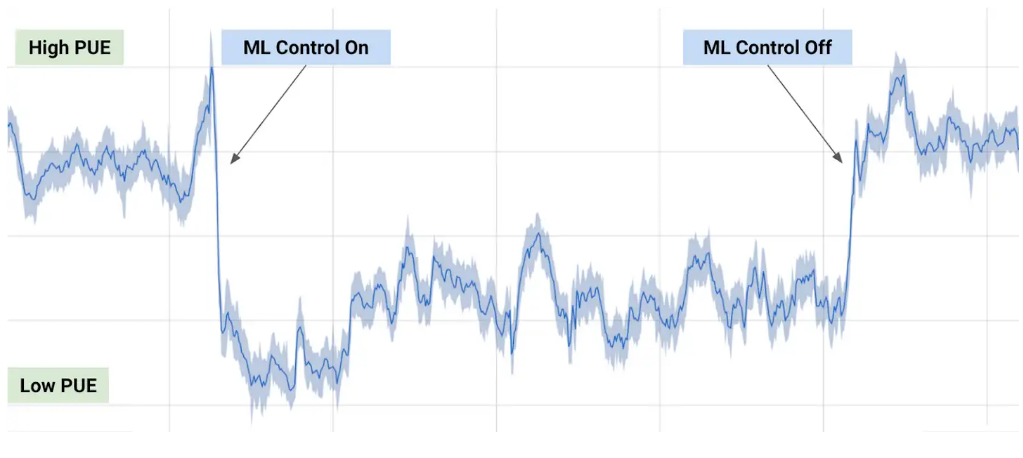
\includegraphics[width=0.7\textwidth]{images/ch5/google_data_center.jpeg}
    \caption{Power usage effectiveness with and without ML control.  Original figure from \cite{google_data1}.}
    \label{fig:google_data_center}
\end{figure}

By 2018, the agent was given full access to the data center control system after safety constraints were added. 

As a summary, the RL agents sample measurements from the sensors in each data center every five minutes and outputs the optimal control actions that satisfy a robust set of safety constraints \cite{google_data2}. The local control operators then verify the provided inputs to ensure that the system will remain within constraint boundaries. In the first few months, the agent consistently reduced electricity consumption by an average of 30\% and is expected to improve as it continues to learn. In the end, the agent reached an optimal policy that resulted in the lowest PUE ever seen, far surpassing human operation---an event only achievable through RL.
